\documentclass[conference]{IEEEtran}
\IEEEoverridecommandlockouts
% The preceding line is only needed to identify funding in the first footnote. If that is unneeded, please comment it out.
\usepackage{cite}
\usepackage{amsmath,amssymb,amsfonts}
\usepackage{algorithmic}
\usepackage[noabbrev,capitalize]{cleveref}
\usepackage{array, booktabs, makecell}
\usepackage{graphicx}
\usepackage{textcomp}
\usepackage{xcolor}
\usepackage{caption}
\usepackage{subcaption}
\newcommand\norm[1]{\left\lVert#1\right\rVert}
\def\BibTeX{{\rm B\kern-.05em{\sc i\kern-.025em b}\kern-.08em
    T\kern-.1667em\lower.7ex\hbox{E}\kern-.125emX}}
\begin{document}

\title{A Deep Learning Approach to Camera Pose Estimation}

\author{\IEEEauthorblockN{Federico Izzo}
\IEEEauthorblockA{\textit{DISI, University of Trento} \\
Trento, Italy\\
federico.izzo@studenti.unitn.it}
\and
\IEEEauthorblockN{Francesco Bozzo}
\IEEEauthorblockA{\textit{DISI, University of Trento} \\
Trento, Italy\\
francesco.bozzo@studenti.unitn.it}
}

\maketitle

% add page number
\thispagestyle{plain}
\pagestyle{plain}

\begin{abstract}
The task of camera pose estimation aims to find the position of the camera that captured an image within a given environment.
While different geometric approaches have already been studied in the literature, the aim of this project is to analyze and improve the performances of deep learning models for the camera pose estimation problem.
In this work, we analyze models for both relative camera pose estimation (MeNet) and absolute camera pose estimation (PoseNet, MapNet). Moreover, we propose a pipeline for the generation of a ground truth dataset based on structure from motion techniques (COLMAP).
Finally, we (1) show how the proposed framework has been used to build a dataset of the second floor of the Povo 1 building in the University of Trento, (2) train an absolute pose estimation model with PyTorch, and (3) deploy it through a web dashboard using FastAPI.
The deep learning approach could give interesting results in combination with geometric methods, especially for: relocation after lost tracking, closed-loop detection, better dealing with moving objects in the scene. Even if the SOTA deep learning approach for this field is less accurate than geometric ones, it ensures more generalization capabilities at a reduced  computational cost.
\end{abstract}

\begin{IEEEkeywords}
camera pose estimation, PoseNet, MapNet, deep learning, computer vision
\end{IEEEkeywords}

\section{Introduction}
The \emph{camera pose}, referenced also with \emph{camera extrinsics}, can be expressed as a combination of two components:
\begin{enumerate}
    \item a tuple of three elements that identifies the absolute coordinates $x,y\text{ and }z$ in a reference space:
          \begin{equation}
              x_c=(x,y,z)\quad x,y,z \in \mathbb{R}
              \label{eq:absolute-position-definition}
          \end{equation}
    \item a quaternion of four elements that identifies the rotation of the camera:
          \begin{equation}
              q_c=(qw, qx, qy, qz)\quad qw,qx,qy,qz \in \mathbb{R}
              \label{eq:quaternion-as-rotation-definition}
          \end{equation}

\end{enumerate}
Consequentially, the pose is referred as $p_c=(x_c, q_c)$.

It is important to notice that this is not the only available representation of a pose: other methods are based also on rotation matrices and Euler angles. It is worth specifying that even if Euler angles are the most straightforward and efficient in terms of memory consumption, they suffer from of the Gimbal lock problem. Even if rotation matrices guarantee a good representation, they are more memory expensive (9 values) than quaternions (only 4 values): for this reason the latter form is preferred here.

Given an image $I_c$ captured by a camera $C$, an absolute pose estimator $E$ tries to predict the $3D$ pose orientation and location of $C$ in world coordinates, defined for some arbitrary reference $3D$ model. The \emph{absolute pose estimation (APE)} problem can be formally defined as the problem of estimating a function $E$ taking as input an image $I_c$ captured by a camera $C$ and as output its respective pose:
\begin{equation}
    E(I_c) = (x_c, q_c)
    \label{eq:absolute-pose-estimation-task}
\end{equation}

\begin{figure}[h]
    \begin{center}
        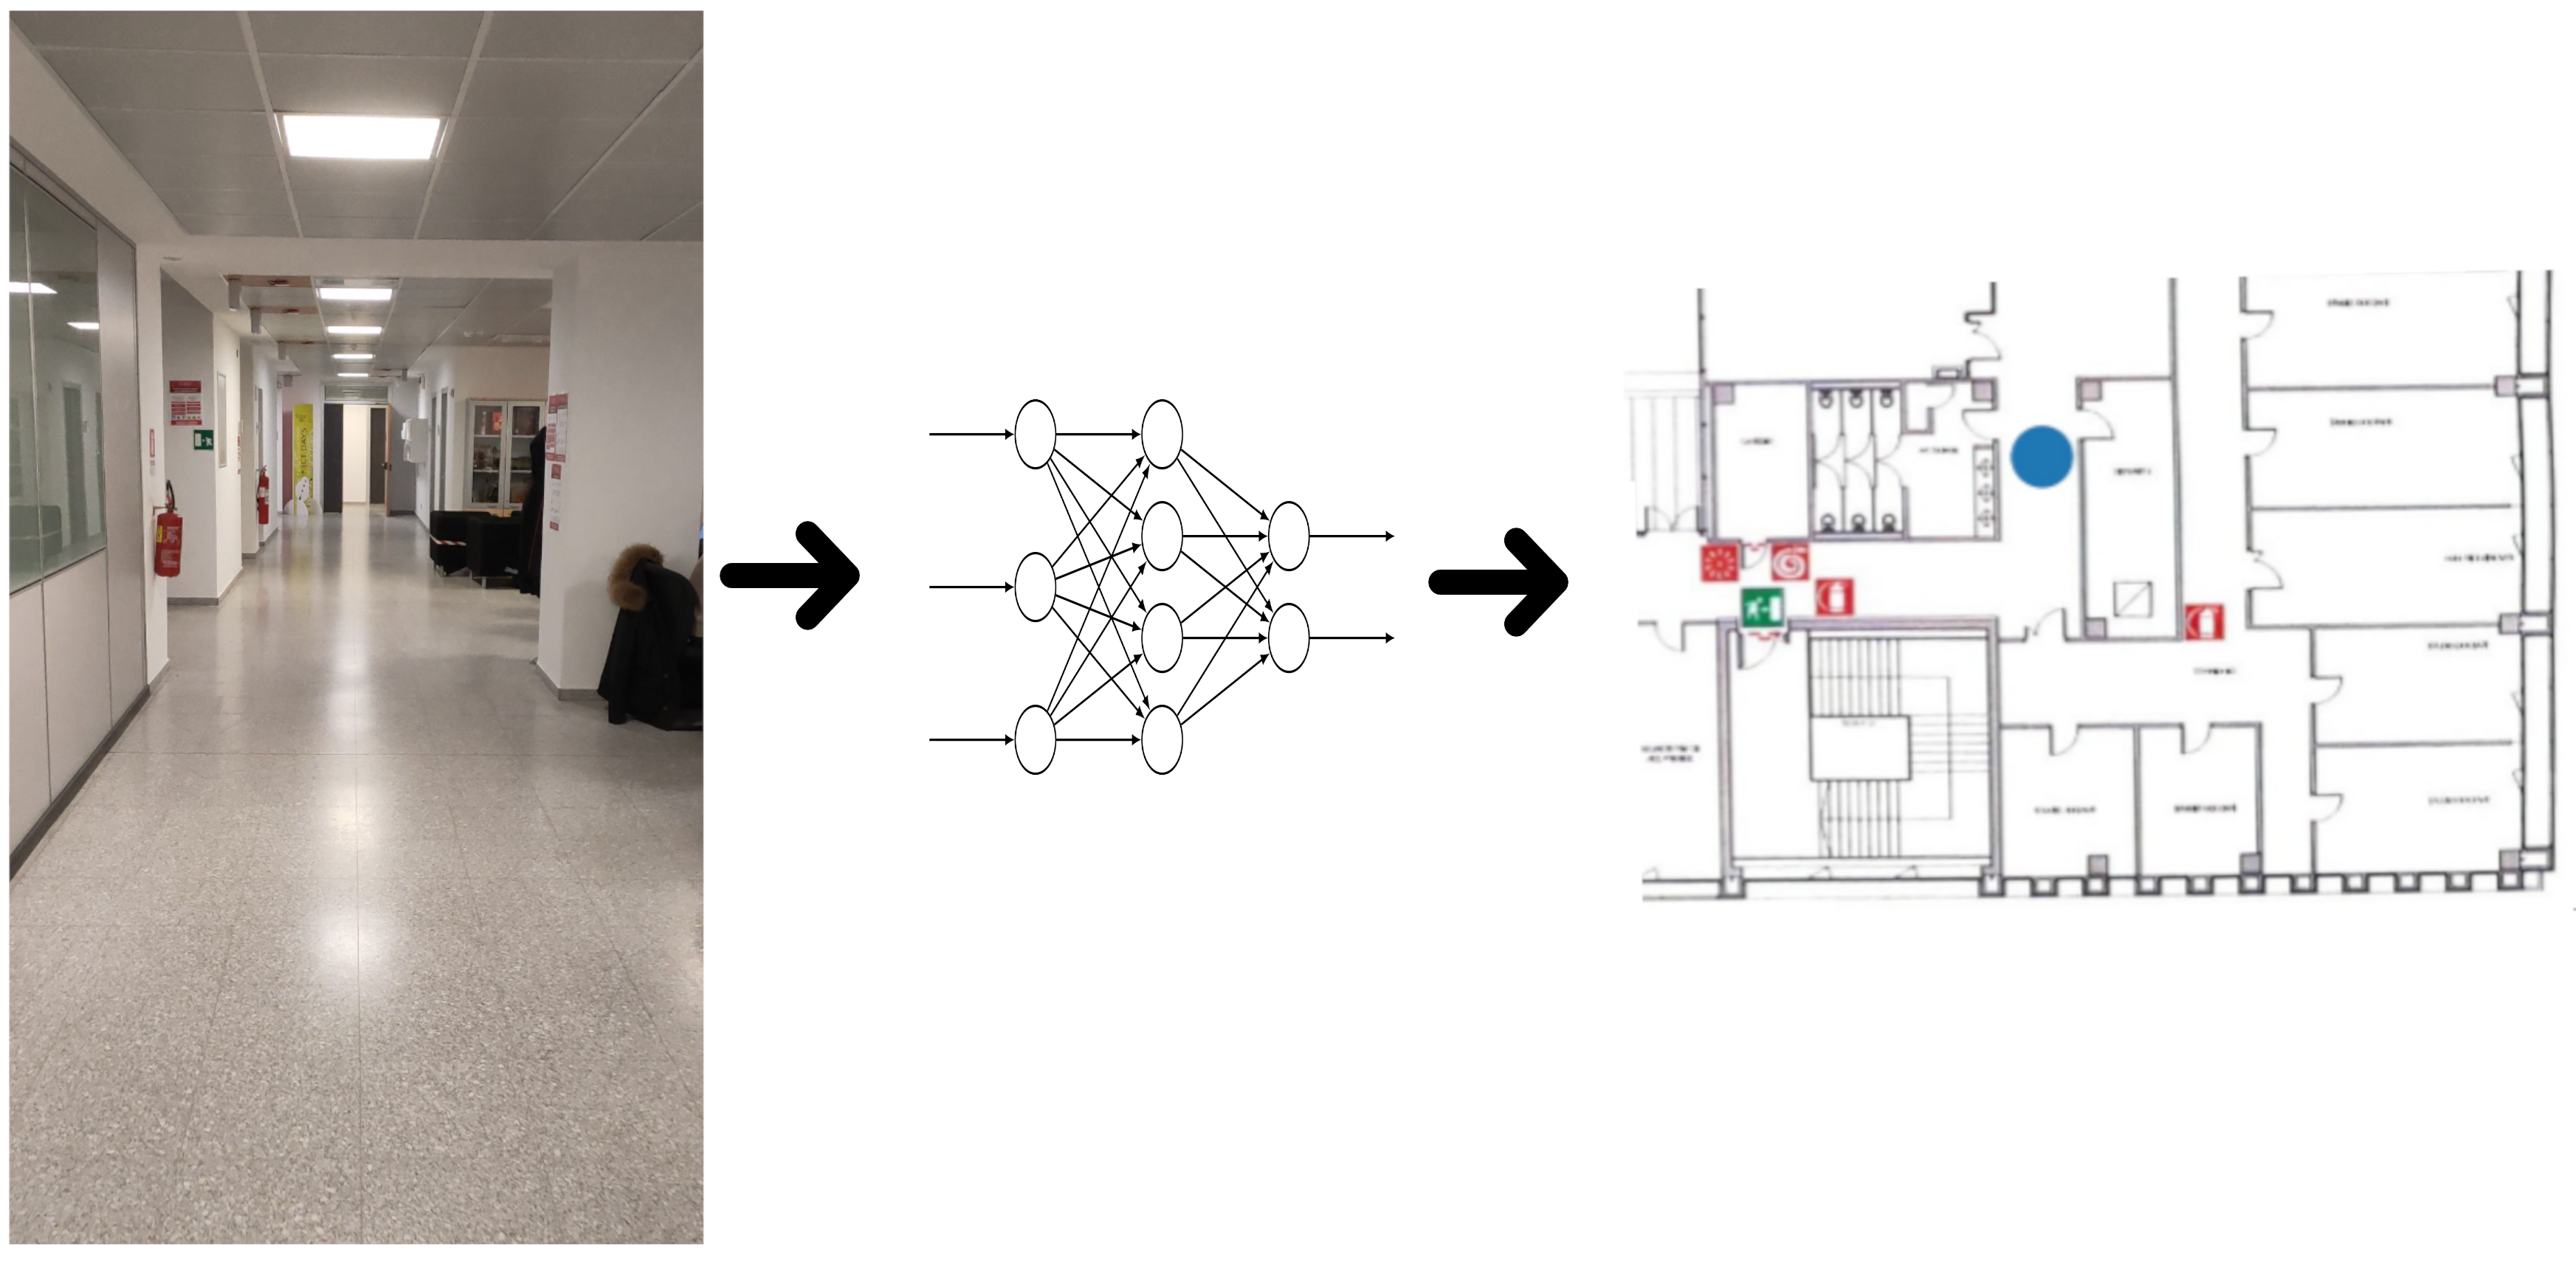
\includegraphics[width=0.48\textwidth]{./imgs/introduction_example.png}
    \end{center}
    \caption{APE model developed}
    \label{fig:introduction-example}
\end{figure}


Apart from APE, a popular task is also \emph{relative pose estimation (RPE)}. In this kind of approach the estimator takes two images $I_c^1$ and $I_c^2$ captured by $C$ and aims to predict the relative pose between them. In this case, the formulation of the function $E$ described in \cref{eq:absolute-pose-estimation-task} is a little different, since it receives in input two images:
\begin{equation}
    E(I_c^1, I_c^2) = (x_c^{rel^2}, q_c^{rel})
    \label{eq:relative-pose-estimation-task}
\end{equation}
where $x_c^{rel}$ is defined as the absolute pose with \emph{coordinates reference system} in $I_c^1$ or, in an equivalent way, as the translation vector from $I_c^1$ to $I_C^2$.

With this work, we show how it is possible to build a deep learning model which is able to learn the function $E$ using a data-driven approach.

\section{Related works}
In the literature there are many deep learning approaches used to perform RPE and APE: here we focus on MeNet for the first and PoseNet~\cite{9348762} and MapNet~\cite{mapnet} for the latter, since they can get good results without requiring huge computational costs.

APE deep learning models rely mostly on \emph{transfer learning}: the idea is to use SOTA pre-trained vision models to extract features from images and use them to estimate camera extrinsics.
The PoseNet model has been the first to be developed following this idea. The starting network for the knowledge transfer is a GoogLeNet~\cite{googlenet}, where the softmax classification layer is replaced with a sequence of fully connected layers. Even if the obtained results are decent, the model (1) lacks of generalization when applied to unseen scenes and (2) fails in learning complex environments.

In order to solve these problems, other techniques have been developed, which can be classified in:
\begin{itemize}
    \item \emph{end-to-end} approaches;
    \item \emph{hybrid} approaches.
\end{itemize}

Most of the end-to-end proposed models are based on the PoseNet architecture, with the addition of some components, such as \emph{encoder/decoder blocks}, \emph{linear layers}, and \emph{LSTM blocks}. The most successful model on this category is MapNet, with its related variants MapNet+ and MapNet+PGO~\cite{mapnet}.

On the other hand, hybrid approaches instead try to focus on different support tasks with the goal of helping the final pose prediction. Those techniques rely on unsupervised learning, 3D objects reconstruction and other data extracted with external tools: for these reasons, such methods are not considered in this work.

\section{Dataset generation}
\subsection{Approaches tested}
The deep learning approaches explained in this document are \textit{supervised learning} techniques that require a labeled dataset. Several paths were tested in order to generate this kind of dataset:
\begin{itemize}
    \item \textit{IMU sensors}: usage of gyroscope and accelerometer sensors of a smartphone to estimate the position of the camera during a video given a fixed origin point. 
    \item \textit{digital video}: usage of free online 3 dimensional datasets in which video can be recorder in a digital way.
    \item \textit{motion capture system}: usage of a motion capture system that estimates the camera position following some tracking objects attached to the subject.
    \item \textit{structure from motion techniques}: techniques that compute a sparse and dense reconstruction from a sequence of images.
\end{itemize}

The main problem encountered with IMU sensors was the high noise presents during acquisitions, the final signal was very dirty, and the resolution was not acceptable for the dataset generation. A possible solution could have been the usage of a well calibrated hardware used in other kind of contexts.

Most of the 3 dimensional acquisitions available online for free are acquired with \textit{depth sensors} or \textit{LIDAR sensors}, for this reason although the camera pose estimation would not have presented any errors the images would have been at low quality.

The motion capture system is able to follows the position of the tracked objects with extremely precision, the main problematic remains the associated of poses to video captured from the camera held by the tracked subject. Other difficulties involved the calibration of the tool.

The techniques of structure from motion were invented with the goal of generate structures for which a huge amount of photos is available. The overall idea is to feed the algorithm with data in order to extract feature and build a recomposition of the environment. A step required in order to obtain a result is the estimation of the pose of images. These intermediate requirement have been exploited by us to generate a labeled dataset.

\subsection{Pipeline}
The implemented pipeline require a video captured by any camera, it is not required any calibration of the sensor. It is composed by several steps:
\begin{enumerate}
    \item video split: the captured video is split into many frames; 
    \item structure from motion: images obtained from the previous step are fed into a structure motion tool called \textit{COLMAP};
    \item cross validation dataset: positions obtained during the camera estimation of the reconstruction process are split into three batches: train, validation, test.
\end{enumerate}

\section{Models}
In this work we take in consideration some state-of-the-art deep learning models for camera pose estimation, also with additional small modifications to make them fit better to our use case scenario.
In particular, we present:
\begin{itemize}
    \item MeNet~\cite{menet} for RPE;
    \item PoseNet~\cite{9348762} and MapNet~\cite{mapnet} for APE.
\end{itemize}

\subsection{MeNet}
The first model we would like to discuss is the MeNet model, that is specifically targeted for RPE.
The input of the network consists in a stack of two images: the goal is to estimate the relative pose of the second image with respect to the first one.
As shown in \cref{fig:menet-structure}, the MeNet is composed by nine deep convolutional layers followed by a sequence of linear layers. While the first part of the network covers the role of feature extraction, the last layers are used to combine the extracted features.
\begin{figure}[htbp]
    \begin{center}
        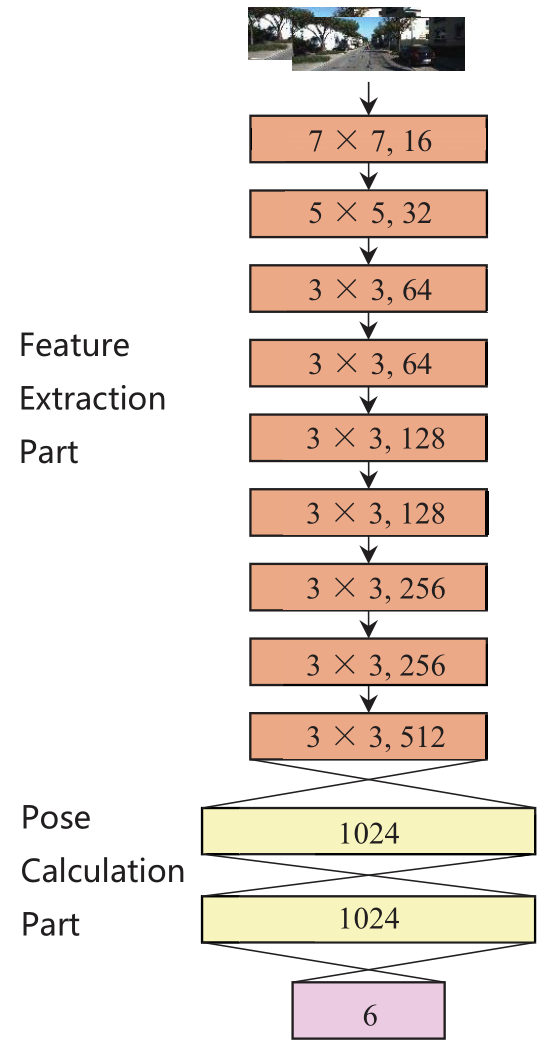
\includegraphics[width=0.32\textwidth]{./imgs/menet_structure.png}
    \end{center}
    \caption{MeNet model architecture.}
    \label{fig:menet-structure}
\end{figure}

In order to train the model, we use a loss function that consists in the weighted composition of two Mean Square Errors (MSE) computed separately on positions and quaternions:
\begin{equation}
    Loss(w) = \frac{1}{N} \sum\limits_{i=1}^N \norm{P^i - \hat{P}^i}^2_2 + \alpha\norm{Q^i - \hat{Q}^i}^2_2
    \label{eq:menet-loss}
\end{equation}
where $P$, $\hat{P}$, $Q$, $\hat{Q}$, and $\alpha$ are the ground truth position vector, the estimated position vector, the ground truth quaternions, the estimated quaternions, and the weight for balancing the displacement error and the rotation angle error.

\subsection{PoseNet}
Since the results given by RPE deep learning solutions are not very promising due to the lack of generalization and to cumulative errors in the estimations, from now on we are going to consider only models strictly developed for APE.
In this sense, the first one we present is the PoseNet model~\cite{9348762}.
As shown in \cref{fig:mapnet-posenet-structure}, just like the MeNet model, the PoseNet is made up by two components:
\begin{itemize}
    \item feature extraction through a sequence of convolutional layers. This component has been named internally also as \emph{backend};
    \item pose regression on the extracted features using linear layers.
\end{itemize}

\begin{figure}[htbp]
    \begin{center}
        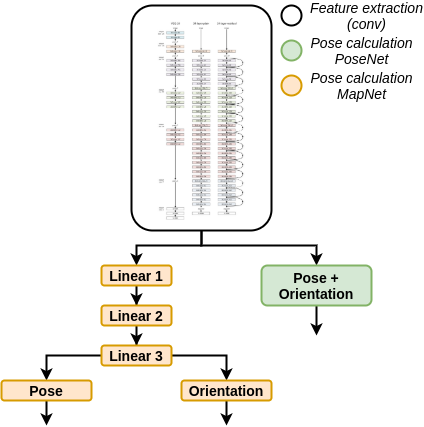
\includegraphics[width=0.32\textwidth]{./imgs/mapnet_posenet_structure.png}
    \end{center}
    \caption{PoseNet and MapNet model architecture.}
    \label{fig:mapnet-posenet-structure}
\end{figure}

This model architecture is actually pretty convenient, since it can use pre-trained deep convolutional networks, through the transfer learning approach. In most of the cases, this kind of models are trained on the ImageNet dataset \cite{imagenet}, which counts almost 3.2 million real-world images: this offer good generalization capabilities for the feature extraction task.
It is important to notice that these models have been developed to work on the ImageNet dataset, which consists of RGB 224x224 pixels images: for this reason, any PoseNet input must have the same shape. 
Some examples of state-of-the-art backend models that have been considered are: GoogLeNet~\cite{googlenet}, ResNet~\cite{resnet}, and EfficientNet-B7~\cite{efficientnet}. \Cref{tab:backend-performance-imagenet} shows the accuracy over the k=(1, 5) top predictions for the used backends on the ImageNet dataset.

\begin{table}[htbp]
    \caption{Backends performance in ImageNet}
    \begin{center}
        \begin{tabular}{lrr}
            \toprule
            Model           & Acc@1           & Acc@5           \\
            \midrule
            GoogLeNet       & 69.778          & 89.530          \\
            ResNet-18       & 69.758          & 89.078          \\
            ResNet-34       & 73.314          & 91.420          \\
            ResNet-50       & 76.130          & 92.862          \\
            ResNet-152      & 78.312          & 94.046          \\
            EfficientNet-B7 & \textbf{84.122} & \textbf{96.908} \\
            \bottomrule
        \end{tabular}
        \label{tab:backend-performance-imagenet}
    \end{center}
\end{table}

Since ImageNet pre-trained models are used for classification purposes, we need to remove the last classification-related layers, and use only the convolutional ones for feature extraction. This gives us the opportunity to insert in the PoseNet a feature extraction mechanism on real-world images with minimum effort: training by scratch such models would require a huge amount of computational power.

Moreover, to train the PoseNet we adopt the weighted loss described in \cref{eq:menet-loss}, also used in the MeNet model.

\subsection{MapNet}
The MapNet model for APE represents an evolution of the PoseNet model: in fact, the model architecture remains actually the same, as shown in \cref{fig:mapnet-posenet-structure}. While even in this case the original model has a single linear layer, we introduce a sequence of them, each followed by the RELU activation function. This enables the model to learn more complex scenarios fitting better the data distribution.

Another difference with respect to the PoseNet is the loss function used to train the model. In this case, the errors on the prediction of absolute poses are not the only ones which are penalized: in fact, also errors in the relative poses are taken in consideration. To be able to penalize also relative errors, during the training process the model receives as input a batch of \texttt{step} ($s$) sorted frames, that are separated by \texttt{skip} ($k$) frames in the original video.
\Cref{eq:mapnet-loss} describes the MapNet loss as a mixture of absolute and relative errors regularized by the $\alpha$ hyperparameter: 

\small
\begin{equation}
    L_\mathcal{D}(\Theta) = \sum\limits_{i=1}^{|\mathcal{D}|} h([\hat{P}^i \hat{Q}^i], [P^i Q^i]) + \alpha\sum\limits_{i,j=1, i\neq j}^{|\mathcal{D}|} h([\hat{P}^{ij} \hat{Q}^{ij}], [P^{ij} Q^{ij}])
    \label{eq:mapnet-loss}
\end{equation}
\normalsize
where $[P^{ij} Q^{ij}]$ is the relative camera pose between pose predictions $[P^i Q^i]$ and $[P^j Q^j]$ for images $I^i$ and $I^j$.
$h(\cdot)$ is a function to measure the distance between the predicted camera pose $\hat{P}$ and the ground truth camera pose $P$, defined as:
\small
\begin{equation}
    h([\hat{P}^i \hat{Q}^i], [P^i Q^i]) = \norm{\hat{P}^i-P^i}_1 e^{-\beta} + \beta + \norm{\hat{Q}^i-Q^i}_1 e^{-\gamma} + \gamma
    \label{eq:mapnet-loss-h}
\end{equation}
\normalsize
where $\beta$ and $\gamma$ are the weights that balance the position loss and rotation loss. Both the parameters can be learned as well during the training procedure. $(I^i, I^j)$ are image pairs within each tuple of $s$ images sampled with a gap of $k$ frames from $\mathcal{D}$.

\section{Results}
\subsection{Posenet}
Several pretrained models can be used as features extractor in the PoseNet structure. In \cref{tab:mapnet-backends} are presented the most powerful ones for features extraction tested on the same final linear encoder. The overall trend is similar, this highlights that the extracted features are enough for the task independently from the backbone used.
\begin{table}[htbp]
\caption{PoseNet backend comparison}
\begin{center}
\begin{tabular}{|c|c|c|c|c|c|}
\hline
\textbf{Model}&\textbf{Position err.}&\textbf{Rotation err.}&\textbf{Params}&\textbf{Tr.$^{\mathrm{a}}$ params} \\
\hline
GoogleLeNet     &0.781&0.119&-         &-      \\
ResNet-18       &0.635&0.288&11,180,103&3,591  \\
ResNet-34       &0.632&0.223&21,288,263&3,591  \\
ResNet-50       &0.707&0.191&23,522,375&14,343 \\
ResNet-152      &0.594&0.139&58,158,151&14,343 \\
EfficientNet-B7 &0.817&0.132&63,804,887&17,927 \\
\hline
\multicolumn{4}{l}{$^{\mathrm{a}}$Trainable}
\end{tabular}
\label{tab:posenet-backends}
\end{center}
\end{table}
\subsection{MapNet}
Several pretrained models can be used as features extractor in the MapNet structure. In \cref{tab:mapnet-backends} are presented the most powerful ones for features extraction tested on the same final linear encoder. The overall trend is similar, this highlights that the extracted features are enough for the task independently from the backbone used.
\begin{table}[htbp]
\caption{MapNet backend comparison}
\begin{center}
\begin{tabular}{|c|c|c|c|c|c|}
\hline
\textbf{Model}&\textbf{Position err.}&\textbf{Rotation err.}&\textbf{Params}&\textbf{Tr.$^{\mathrm{a}}$ params} \\
\hline
ResNet-18       &0.202&0.0658&14,853,703&3,677,191 \\
ResNet-34       &0.187&0.0757&24,961,863&3,677,191 \\
ResNet-50       &0.220&0.0969&30,330,951&6,822,919 \\
ResNet-152      &0.233&0.0869&64,966,727&3,677,191 \\
EfficientNet-B7 &0.210&0.0848&71,658,455&7,871,495 \\
\hline
\multicolumn{4}{l}{$^{\mathrm{a}}$Trainable}
\end{tabular}
\label{tab:mapnet-backends}
\end{center}
\end{table}

Another point that emerges is the importance of the final encoder, it works in a similar way of the \textit{bag of words} used by structure from motion (link al paper). Extracted features are mapped in a space that is used later as a comparison tool for new images for which the pose is asked.
For this reason the final encoder was modified from the original one (link al paper) in order to increase the latent space in which data can be stored.

\subsection{Comparison}
\subsection{Dashboard}
A dashboard was developed with the aim to easily allow users to interact with model inference through a webserver. In \cref{fig:dashboard} is presented the \textit{UI} where red zones are not walkable areas.
\begin{figure*}
    \begin{center}
        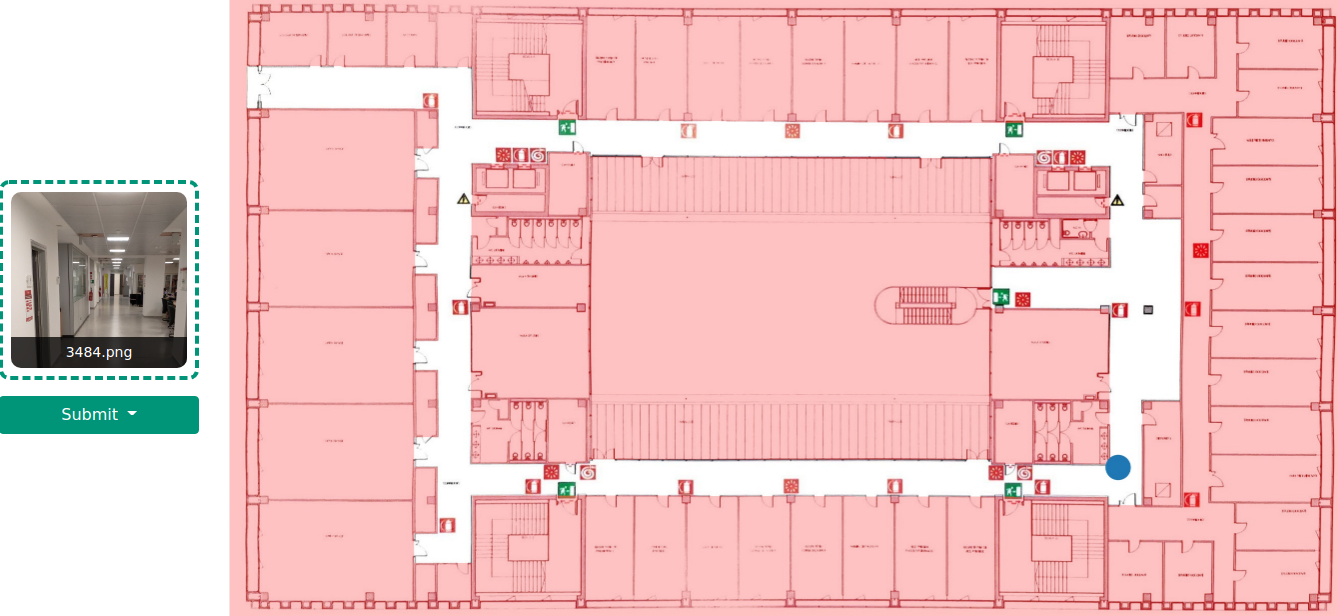
\includegraphics[width=0.95\textwidth]{./imgs/dashboard.png}
    \end{center}
    \caption{Inference dashboard}
    \label{fig:dashboard}
\end{figure*}


% accuracy with respect to different ResNets used. The bigger the ResNet, the better the results should be

% Some accuracies wrt. hyperparameters tuning

% Some plots on losses

\section{Materials}
Every material used in the project have been uploaded respectively:
\begin{itemize}
    \item the datasets have been uploaded on the Google Drive folder;
    \item the code is available in the GitHub repository.
\end{itemize}

The project has been developed in Python 3, using common data science libraries, such as numpy, pandas, PyTorch, matplotlib, scipy, aim and many others.

\subsection{Repository organization}
The repository follows the structure:
\begin{itemize}
    \item \texttt{camera-pose-estimation/}
    \begin{itemize}
        \item \texttt{model/} contains everything related to the deep learning part of the project. It also includes the code used for implementing the web server under \texttt{webserver.py} and \texttt{static/}.
        \item \texttt{tools/} contains scripts used for the dataset generation pipeline.
    \end{itemize}
    \item \texttt{config\_parser/}: Python package written by us that allows to create configuration files, with the idea of improving reproducibility in our experiments. Each configuration file can be subdivided in sections: for each section you can define variables with the sintax \texttt{label=value}, where \texttt{value} is a parsable JSON object (boolean, int, float, list, object).
    \item \texttt{notebooks/} contains some Python Jupyter Notebooks that have been used for data exploration, validation, and post-processing of the model predictions.
\end{itemize}

\subsection{Data organization}
For each footage, a folder has been created:
\begin{itemize}
    \item \texttt{imgs/} contains the video frames exported with ffmpeg;
    \item \texttt{processed\_dataset/} contains the train, validation, and test datasets that can be reused during different trainings: this helps speeding up the loading procedure from \dots minutes to \dots seconds;
    \item \texttt{workspace/} contains the models generated by COLMAP;
    \item each of \texttt{train.csv}, \texttt{validation.csv}, and \texttt{test.csv} contains a table for specifying the pose for each image frame. This are the files generated with the \texttt{video\_to\_dataset.sh} script.
\end{itemize}

\section{Conclusions}
To summarize, the final results presented in this work are:
\begin{itemize}
    \item the exploration of multiple dataset generation techniques;
    \item the COLMAP reconstruction of Povo 1 second floor;
    \item the development of relative and absolute pose estimation models;
    \item the fine-tuning of absolute pose estimation models;
    \item the post-processing of the model outputs;
    \item the model deployment using a FastAPI web-server. 
\end{itemize}

But, even if the proposed results are promising, there are still many things to consider.
Many of the future developments of this work should concentrate on:
\begin{itemize}
    \item trying MapNet+, which is able to learn also from unlabeled data through a semi-supervised approach;
    \item trying MapNet+PGO, which performs pose graph optimization (PGO) during inference time;
    \item modifying the model loss to penalize predictions which are in a non-walkable area;
    \item testing the models in an outdoor environment, with different weather conditions;
    \item automatizing the coordinate reference system alignment procedure;
    \item build a more robust indoor dataset to validate the full potential of the proposed deep learning approach;
    \item deploy the model to the end-user device to ensure privacy and reduce latency.
\end{itemize}


\bibliography{bibliography.bib}{}
\bibliographystyle{IEEEtran}

\end{document}
